\documentclass[10pt]{article}
%Gummi|063|=)
\usepackage{times}
\usepackage[T1]{fontenc}
\usepackage{etoolbox}
\usepackage{graphicx}
\usepackage{subfigure}
\usepackage[english]{babel}
\usepackage{geometry}
 \geometry{
 a4paper,
 total={170mm,257mm},
 left=20mm,
 top=20mm,
 }
\usepackage{cite}

\title{\textbf{Performance Analysis Of MPI Over Cluster}}
\author{Achuth PV, 133079007\\
		Anirudh Rao, 133079005\\
		Avishkar P, 143070037}
\date{}
\begin{document}

\maketitle

\section{Introduction}

Clusters are widely used in the field of high performance computing to scale  computing beyond a single node. In these cluster, multiple nodes connected via communication networks share the computation load, thus giving scalability and speed up. But, the communication networks between these nodes have always been a major bottleneck in the performance and scalability of these high performance clusters.

There are multiple types of communication networks used in these clusters. Some examples are: Ethernet, Myrinet, InfiniBand, etc. Nodes communicate via these networks using various message passing systems, with message passing interface (MPI) as one of the standardized and commonly used systems.

Ethernet is the most widely LAN technology. It works using TCP/IP stack and  is based on IEEE 802.3 stadard. It supports a wide range of connectors and has good interoperability and is cheap. 

InfiniBand (IB) is a communication architecture which is used for low latency and high bandwidth inter-server communication~\cite{pfister2001introduction}. It was developed as part of Open Fabrics Alliance. It is highly reliable, scalable and has very good performance. Unlike Ethernet based systems which runs algorithm on CPU, the IB adapter can handle network protocol itself, thus freeing up CPU and OS, as well as bypassing multiple system calls. Depending upon the PCI-e technology node's motherboard supports, the performance of InfiniBand network changes. 

MPI can be used with CUDA as CUDA over MPI to utilize the GPU cards residing in multiple nodes in a cluster. The communication bottle neck in this method is that, for each data transfer between machines, data has to be moved from the device to the host memory and then use MPI to transer the data between machines. The data is then copied to device from host at the receiving node. CUDA-Aware MPI~\cite{cudaaware,cheng2014professional} is used to reduce this overhead. It uses unified virtual addressing (UVA) feature, available in CUDA cards with compute capability 2.0 and later, and CUDA 4.0 and later, which combines the host memory and memory of GPUs within a system as one large virtual address space. CUDA-Aware MPI thus supports transferring GPU buffers which exists on a particular machine's GPU card to other machine's GPU card directly, without using host buffer. This reduces many overheads and thus increases communication bandwidth between GPU cards over network. Thus it is easy to pipeline all operations requiring message transfer. Also features like GPU direct can be used by MPI libraries to speed up the communication, by bypassing multiple hardware level overheads. 

In this project, We intend to evaluate various communication platforms available for parallel computing/ cluster computing. We evaluate different MPI implementations, CUDA, CUDA-Aware MPI techniques over different network setup like Ethernet, IP over InfiniBand and shared memory. For this purpose, we use a matrix multiplication program, with matrix size varied from 2000x2000 to 10000x10000, and plot the various computation and data transfer times. The plots are used to evaluate and provide inferences.There are 2 open implementations of MPI available, which support InfiniBand communication along with Ethernet Viz. OpenMPI and MVAPICH2. Both these implementations also support CUDA-Aware MPI technique. We use these two implementations for our evaluation.


\section{Tools and Methods}
\label{methods}

For our work, we used the following tools: OpenMPI and MVAPICH2.
Both of them implement MPI standards. OpenMPI targets certain common usages, while MVAPICH2 is an extension of MPICH, which is the standard MPI implementation. Both of them support lots of communication interfaces like InfiniBand, Ethernet, etc. They also support CUDA-Aware MPI.






Our test code, matrix multiplication was performed using OpenMPI and MVAPICH2 over a cluster of 2 machines connected using InfiniBand as well as Ethernet. This test program was run with different matrix sizes, different number of processes per node and different modes of communication.

Using OpenMPI, MVAPICH2 implementation, the following combination of the code was run:
\begin{enumerate}
\item OpenMPI with matrix size 2000,4000,6000,8000,10000 on single node with 8,16 processes
\item OpenMPI with matrix size 2000,4000,6000,8000,10000 on two nodes with 8,16,32 processes and communication between hosts through Ethernet
\item OpenMPI with matrix size 2000,4000,6000,8000,10000 on two nodes with 8,16,32 processes and communication between hosts through InfiniBand
\item MVAPICH2 with matrix size 2000,4000,6000,8000,10000 on single node with 8,16 processes
\item MVAPICH2 with matrix size 2000,4000,6000,8000,10000 on two nodes with 8,16,32 processes and communication between hosts through Ethernet
\item MVAPICH2 with matrix size 2000,4000,6000,8000,10000 on two nodes with 8,16,32 processes and communication between hosts through InfiniBand
\end{enumerate}


To check the performance of CUDA-Aware MPI, we setup a CUDA cluster. We installed OpenMPI and MVAPICH2 on this cluster. Codes for both the CUDA over MPI and CUDA-Aware MPI are written such that, they send messages of lengths from 1 Byte to 4 MB between two MPI processes. In the CUDA over MPI case, we use  pinned host memory to communicate between the host and the device, thus speeding up host-device communication. We used non-blocking method for communication. 
Two methods are used for evaluation:
\begin{enumerate}
\item Two processes are run on same node.
\item Two processes are run on separate nodes.
\end{enumerate}  
Bandwidth for different message sizes are used for performance  evaluation.

\section{Details of Infiniband Cluster}
\begin{itemize}
\item Number of machines: 14 -  2 masters, 12 slaves
\item Filesystem: GlusterFS
\item OS: CentOS release 6.5 (Final)
\item CPU: Intel(R) Xeon(R) CPU E5-2670 0 @ 2.60GHz
\begin{itemize}
\item 2 CPUs: NUMA with 8 cores/each, 1 thread/core
\item Cache: L1d - 32K, L1i - 32K, L2 : 256K, L3 : 20480K
\end{itemize}
\item 64GB RAM
\item OpenMPI Version : 1.8.4
\item MVAPICH2 Version: 2.1
\item InfiniBand card: QLogic Corp. IBA7322 QDR InfiniBand HCA
\item Infiniband switch : QLogic 12200-18 36-ports
\item Link speed: 40 Gb/sec (4X QDR)
\item Ethernet controller: Intel Corporation I350 Gigabit Network Connection
\end{itemize}
For more details about CPU and memory, please refer Infiniband\textunderscore CPU\textunderscore details.txt and Infiniband\textunderscore Memory\textunderscore details.txt.

\section{Details of CUDA Cluster}
We setup a CUDA cluster of 4 machines. All the machines are Dell Optiplex 3020 with the following specifications
\begin{itemize}
\item 4 Machines
\item Ubuntu 12.04 64 bit
\item Intel(R) Core(TM) i3-4130 CPU @ 3.40GHz
\begin{itemize}
\item 2 cores, 2 threads each
\item Cache - 128kB L1, 512kB L2,  3MB L3 
\end{itemize}
\item 4 GB RAM
\item GeForce GT 640
\begin{itemize}
\item CUDA cores 384 
\item 2048 MB RAM
\item Memory clock rate: 891 Mhz
\item Memory bus width: 128-bit
\item GPU clock rate: 902 MHz 

\end{itemize}
\item CUDA Toolkit 6.5
\item 500 GB harddisk 
\item Ethernet controller: Realtek Semiconductor Co., Ltd. RTL8111/8168/8411
\item OpenMPI: 1.8.8
\item MVAPICH2: 2.1
\end{itemize}

To set up the CUDA cluster, following steps were followed:
\begin{itemize}
\item A file based partitions is created~\cite{filebased}
\item A NFS server is setup on the same machine, sharing the file based partition~\cite{nfssetup}
\item An user account 'mpiuser' is created on the machine with the NFS partition containing its home
\item The NFS partition is mounted on other machines on the cluster
\item The same 'mpiuser' with same gid and uid are created on all the machines, with the same home folder location as earlier.
\item After logging in as 'mpiuser', SSH key is generated and added to authorized\textunderscore keys file
\item All the desired machines for communication are added into known\textunderscore hosts 
\item Both MVAPICH2~\cite{mvapich} and openmpi~\cite{openmpi} versions supporting CUDA-aware MPI are downloaded, built and installed on the home folder 
\end{itemize}

\section{Plots for MPI}
Using the methods discussed in Section~\ref{method}, performance evaluation is done for all the cases. The data obtained is then plotted using MATLAB for performance analysis.

The flow for our test code in MPI invovles : 
\begin{enumerate}
\item Broadcast B matrix to all nodes.
\item Send parts of A from master process (process 0) to other processs (within same node and also to another node).
\item Computation assigned to each process
\item Send back part od C computed at each process to master process.
\end{enumerate}
Three out of four steps in the code involves communication. We have recorded timings of each of these steps to evaluate the performance for different combinations of methods of communication, matrix size, number of processes and different implementations of MPI.
The plots are made with fixed number of processes, for varying size of matrices to evaluate performance of different methods of communication in parallel programming and different implementations of MPI which is our main goal.

First set of plots give timings for entire code. Second set of plots give time taken to broadcast B. Third set of plots give time taken to transfer parts of A. Last and final set of plots give the time taken to transfer back computed matrix C.



\begin{figure*}[p]
\centering
        \subfigure{%
        	\centering
            \label{alignM}
            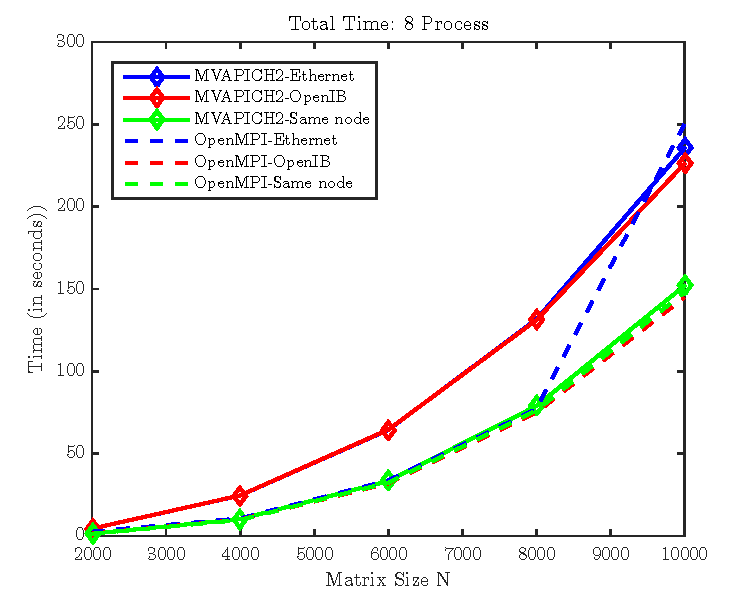
\includegraphics[width=0.45\textwidth]{figure/full_8.pdf}
        }
        ~
        \subfigure{%
           \label{alignB}
           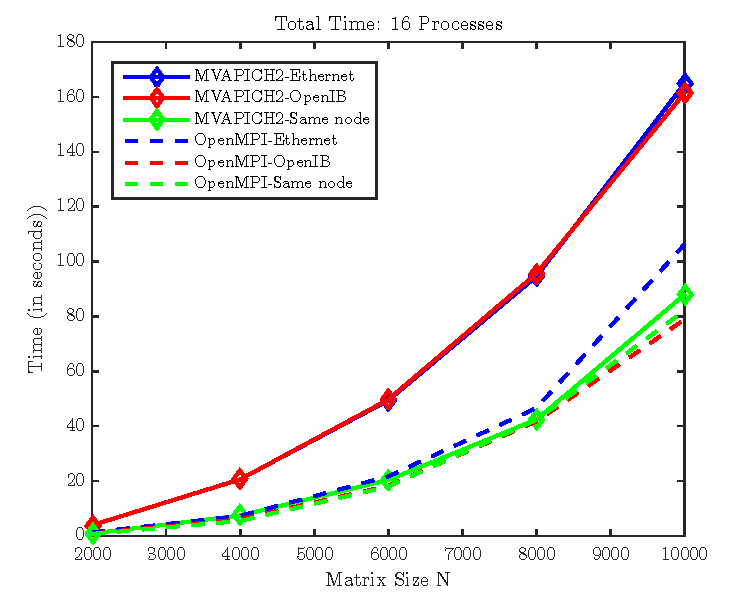
\includegraphics[width=0.45\textwidth]{figure/full_16.pdf}
        }
        \subfigure{%
        	\centering
            \label{shiftM}
            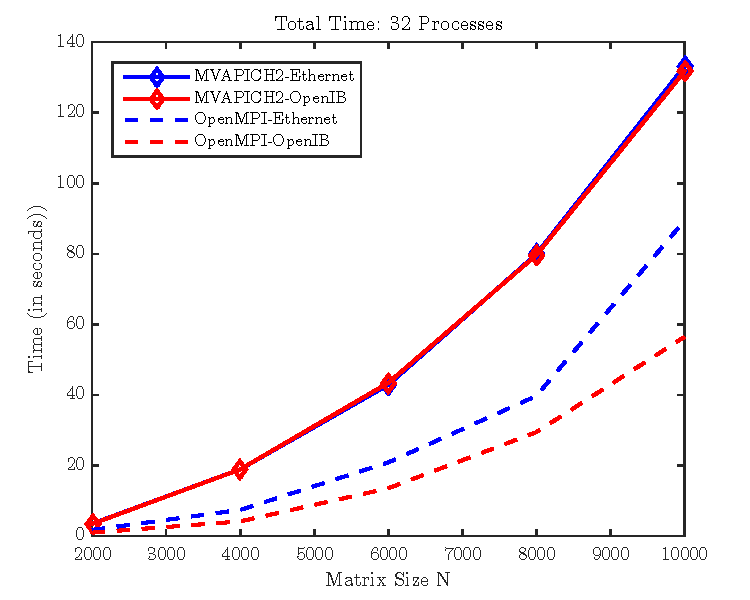
\includegraphics[width=0.45\textwidth]{figure/full_32.pdf}
        }
    \caption{Comparison of Total Time taken for 8, 16 and 32 processes}
   \label{totaltime}
\end{figure*}

\begin{figure*}[p]
\centering
        \subfigure{%
        	\centering
            \label{alignM}
            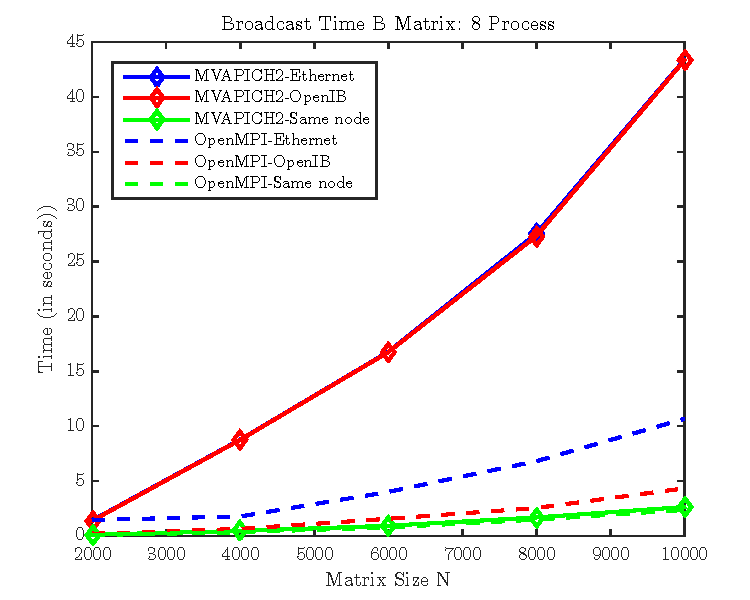
\includegraphics[width=0.45\textwidth]{figure/bcast_8.pdf}
        }
        ~
        \subfigure{%
           \label{alignB}
           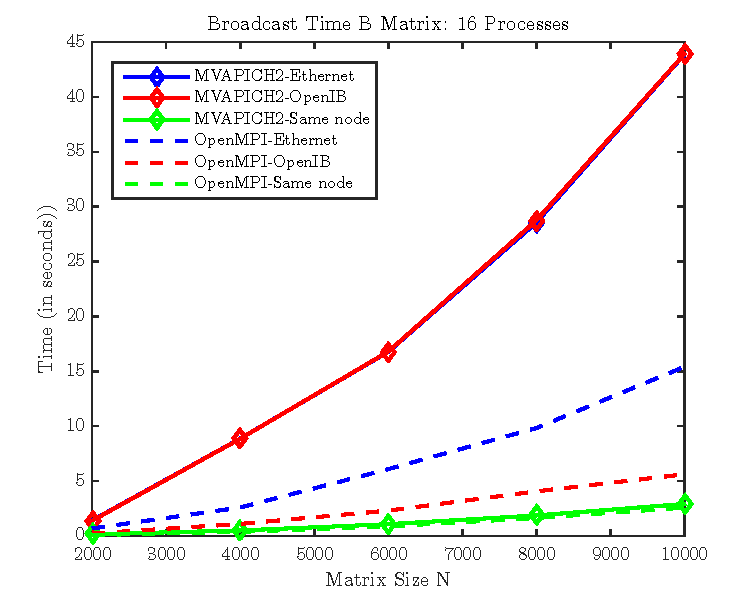
\includegraphics[width=0.45\textwidth]{figure/bcast_16.pdf}
        }
        \subfigure{%
        	\centering
            \label{shiftM}
            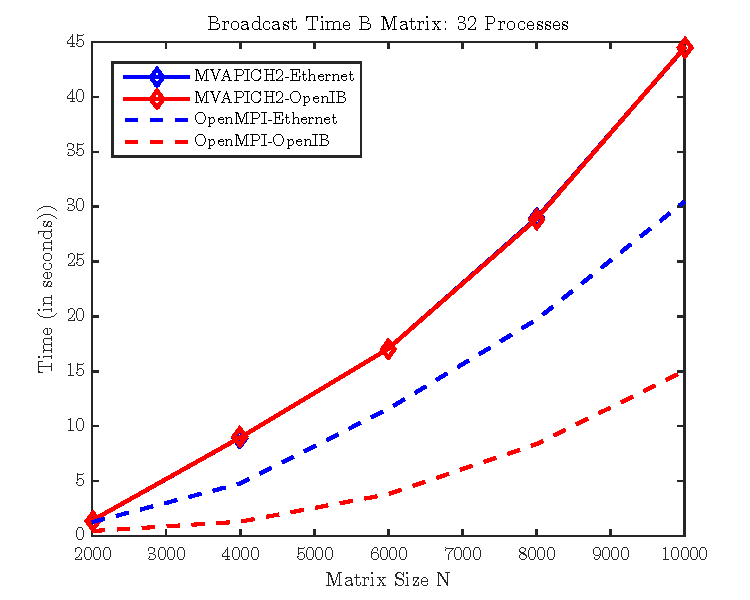
\includegraphics[width=0.45\textwidth]{figure/bcast_32.pdf}
        }
    \caption{Comparison of Broadcast Time taken for matrix B for 8, 16 and 32 processes}
   \label{broadcast}
\end{figure*}

\begin{figure*}[p]
\centering
        \subfigure{%
        	\centering
            \label{alignM}
            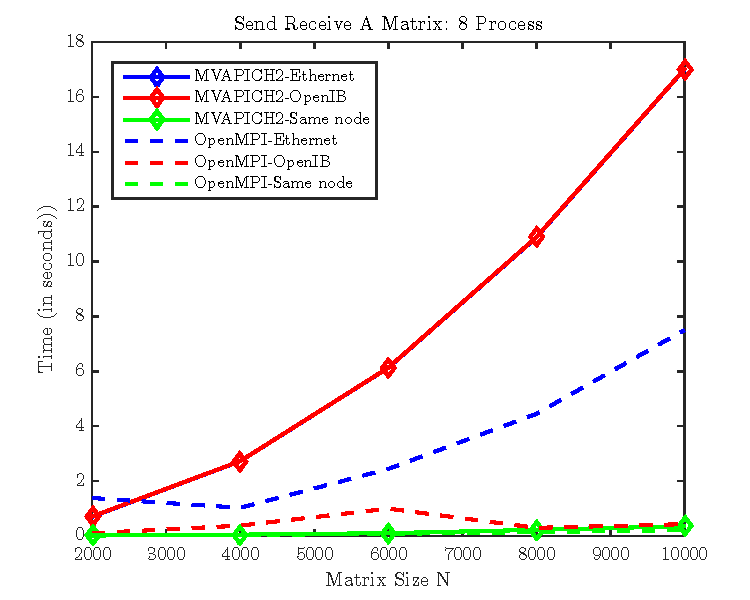
\includegraphics[width=0.45\textwidth]{figure/sendrecvA_8.pdf}
        }
        ~
        \subfigure{%
           \label{alignB}
           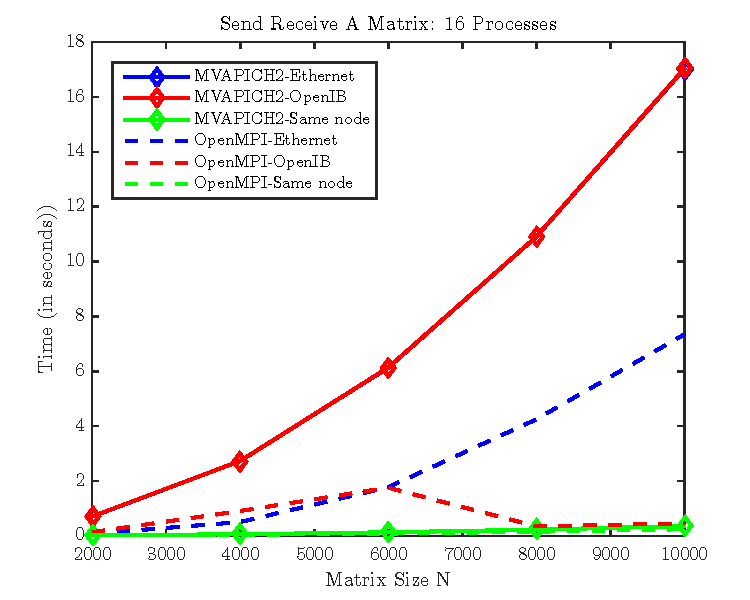
\includegraphics[width=0.45\textwidth]{figure/sendrecvA_16.pdf}
        }
        \subfigure{%
        	\centering
            \label{shiftM}
            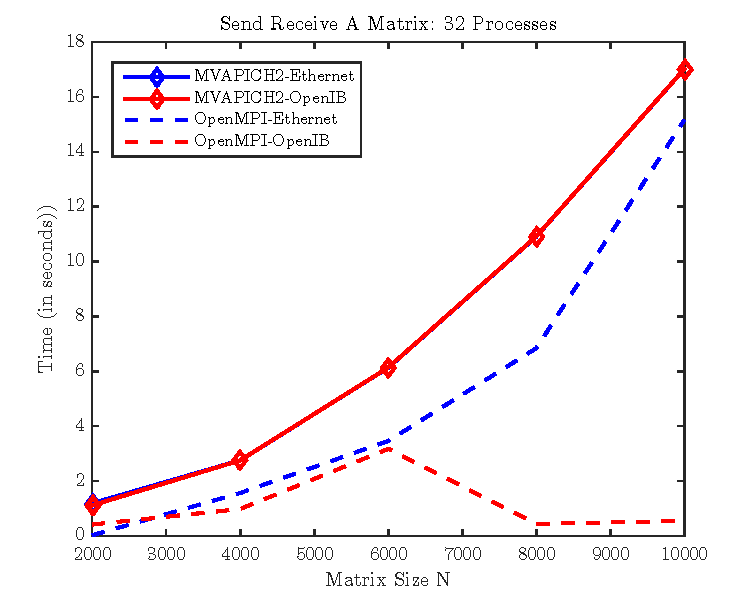
\includegraphics[width=0.45\textwidth]{figure/sendrecvA_32.pdf}
        }
    \caption{Comparison of Send-Receive Time taken for matrix A for 8, 16 and 32 processes}
   \label{sendrecvA}
\end{figure*}


\begin{figure*}[p]
\centering
        \subfigure{%
        	\centering
            \label{alignM}
            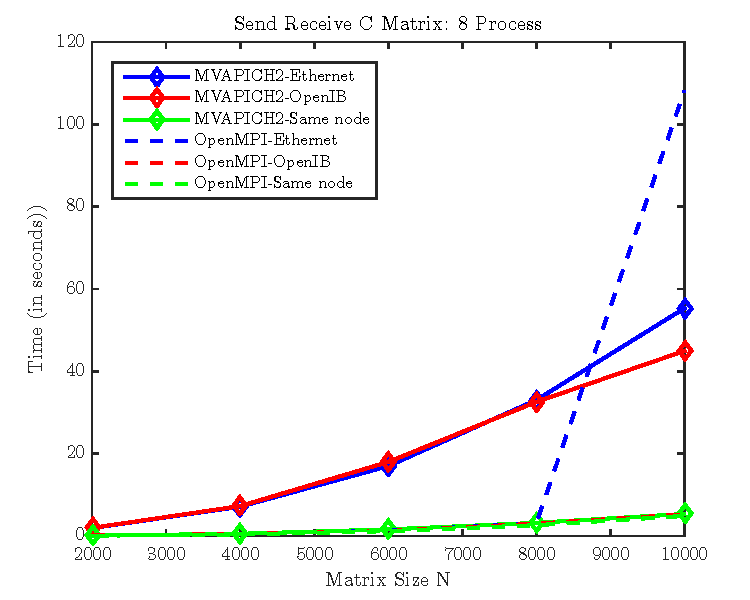
\includegraphics[width=0.45\textwidth]{figure/sendrecvC_8.pdf}
        }
        ~
        \subfigure{%
           \label{alignB}
           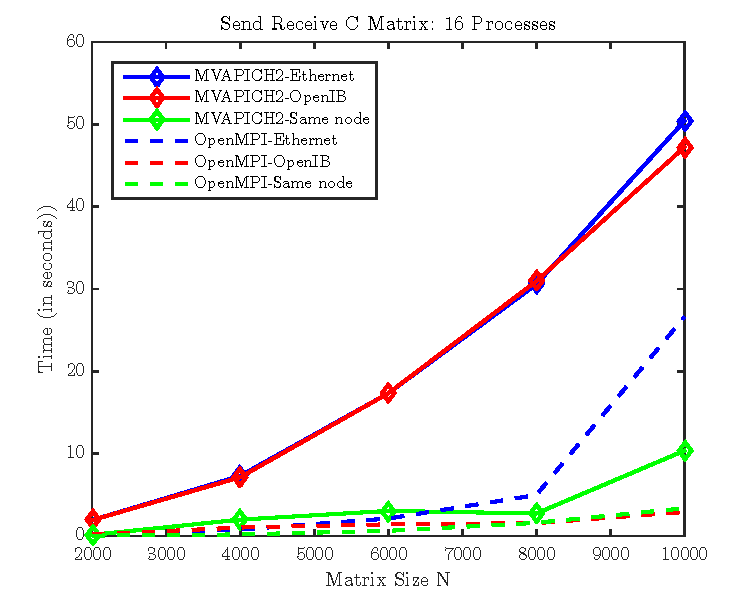
\includegraphics[width=0.45\textwidth]{figure/sendrecvC_16.pdf}
        }
        \subfigure{%
        	\centering
            \label{shiftM}
            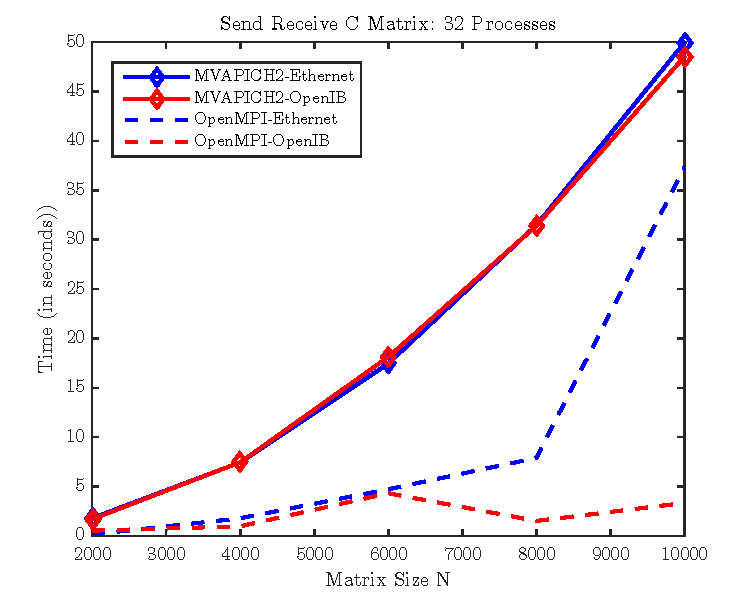
\includegraphics[width=0.45\textwidth]{figure/sendrecvC_32.pdf}
        }
    \caption{Comparison of Send-Receive Time taken for matrix C for 8, 16 and 32 processes}
   \label{sendrecvC}
\end{figure*}

\begin{figure*}[p]
\centering
        \subfigure{%
        	\centering
            \label{alignM}
            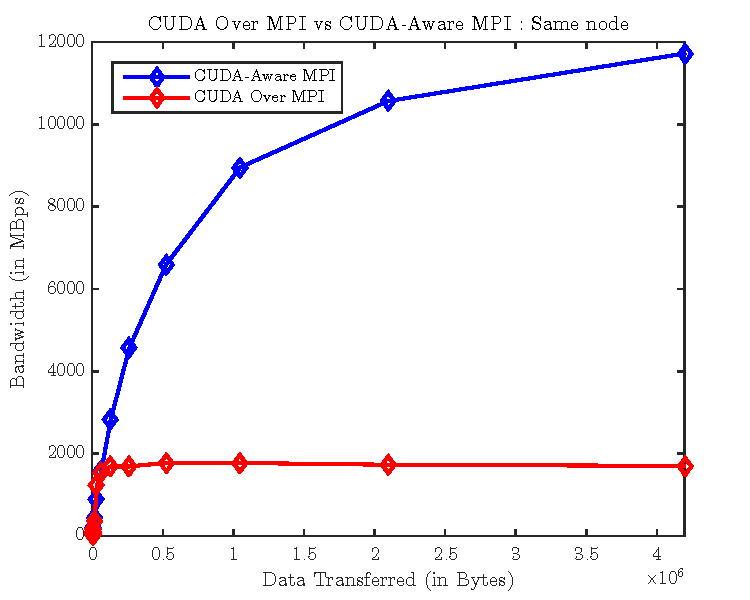
\includegraphics[width=0.45\textwidth]{figure/C_Same.pdf}
        }
        ~
        \subfigure{%
           \label{alignB}
           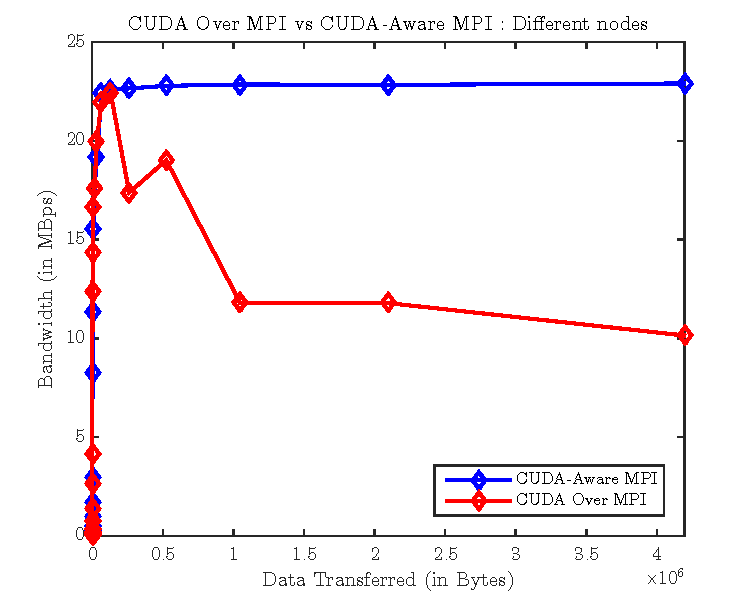
\includegraphics[width=0.45\textwidth]{figure/C_Diff.pdf}
        }
      
    \caption{Comparison of CUDA-Aware and CUDA over MPI for same and different nodes}
   \label{cuda}
\end{figure*}

\subsection{Observations and Inferences}

\begin{enumerate}
\item MPI run over InfiniBand communication takes far lesser time than Ethernet based communication. This is obvious as InfiniBand has higher data rates compared to Ethernet. This performance boost can be significantly seen in OpenMPI but not so much in MVAPICH2.

\item Communication to other processes within the same machine is faster compared to communication over Ethernet. Generally, interprocess communication is very fast compared to Ethernet communication. There is a significant difference in the time taken for these two methods of communication that can be observed in the plots.
 
\item The time taken for intra node inter process communications is comparable to the time taken for InfiniBand communication. InfiniBand provides very high data rates of upto 40Gbps. For smaller size of matrix i.e lesser number of bytes to be transferred, these speeds are comparable to the inter process communication. But for larger size of matrix, intra node inter process communication may perform significantly better

\item With increase in the number of processes and fixed matrix size, the computation time per node decreases; but the time taken for communication remains almost the same. This is because, the major communication is the time taken to broadcast B which remains same as the matrix size is not changed. There may be slight variations in time due to the change in the fraction of A, and C transfered between devices.

\item For a fixed number of processes, as matrix size increases, both computation time and communication time increases almost linearly. This is because, as the size of matrix increases, the number of computations per node/process increases. Also the number of bytes of data to be transmitted from/to a process also increases.
 
\item Comparing the two implementations of MPI, we see that OpenMPI has a better performance compared to MVAPICH2. Also we see that in case of MVAPICH2, there is no much difference in performance when we switch from Ethernet to InfiniBand for communication. The reason still unclear, may also be a configuration issue in the cluster.
\end{enumerate}

As shown in Figure~\ref{cuda}, it can be seen that, CUDA-Aware MPI out performs CUDA over MPI, for both test cases. There is a performance difference of  10 times for messages of length 4 MB for the same node test case. This is because of the overcoming of overhead provided by CUDA over MPI, where the host to device and device  to host communication becomes an overhead. This overhead is not there for the CUDA-Aware MPI case.  For the second test case, the 1GB network of the cluster becomes a bottleneck, resulting the saturation of speed.

\AtEndEnvironment{thebibliography}{

\bibitem{filebased} File based partition, https://www.debuntu.org/how-to-create-a-filesystem-within-another-partitions-file
\bibitem{nfssetup} NFS Setup, https://www.digitalocean.com/community/tutorials/how-to-set-up-an-nfs-mount-on-ubuntu-12-04
\bibitem{mvapich} MVAPICH2-2.1, http://mvapich.cse.ohio-state.edu/static/media/mvapich/mvapich2-2.1-userguide.html
\bibitem{openmpi} OpenMPI, https://www.open-mpi.org/faq/?category=buildcuda

\bibitem{cudaaware} CUDA-Aware MPI, https://devblogs.nvidia.com/parallelforall/introduction-cuda-aware-mpi/
}
\bibliographystyle{plain}
\bibliography{te.bib}{}
\bibliographystyle{plain}


\end{document}
